


\section{Design and Implementation}

\subsection{Overview of the SSDTrain System}\label{sec:ssdtrain_overview}
SSDTrain implements a {\it tensor cache} to \kwc{manage} the offloading and reloading of tensors, facilitating the release of memory and the prefetch of tensors back to memory before they are needed for backward propagation. 
Figure~\ref{fig:pipe} demonstrates how SSDTrain works using PyTorch as an example.
SSDTrain launches its threads~(separate from PyTorch's execution threads) to store tensors~(\textcircled{1}) and to load them back~(\textcircled{5}). In forward propagation~(F), offloading of an activation starts once the operator producing it finishes~(\textcircled{1}). When activations are reused in backward propagation~(B), prefetching~(\textcircled{5}) occurs in the reverse order of layers as recorded during forward propagation~(\textcircled{2}). \kwc{If the last layer begins backward propagation immediately after its forward propagation}~(L3 \kwc{in micro-batch 2} in the example) , \kwc{SSDTrain} keeps the layer's activations \kwc{in GPU memory} instead of offloading them~(\textcircled{4}). SSDTrain keeps individual records for each micro-batch. Upon micro-batch changes~(\textcircled{2}), SSDTrain switches its record to the one corresponding to the new micro-batch. 


\begin{figure}[!t]
\centering
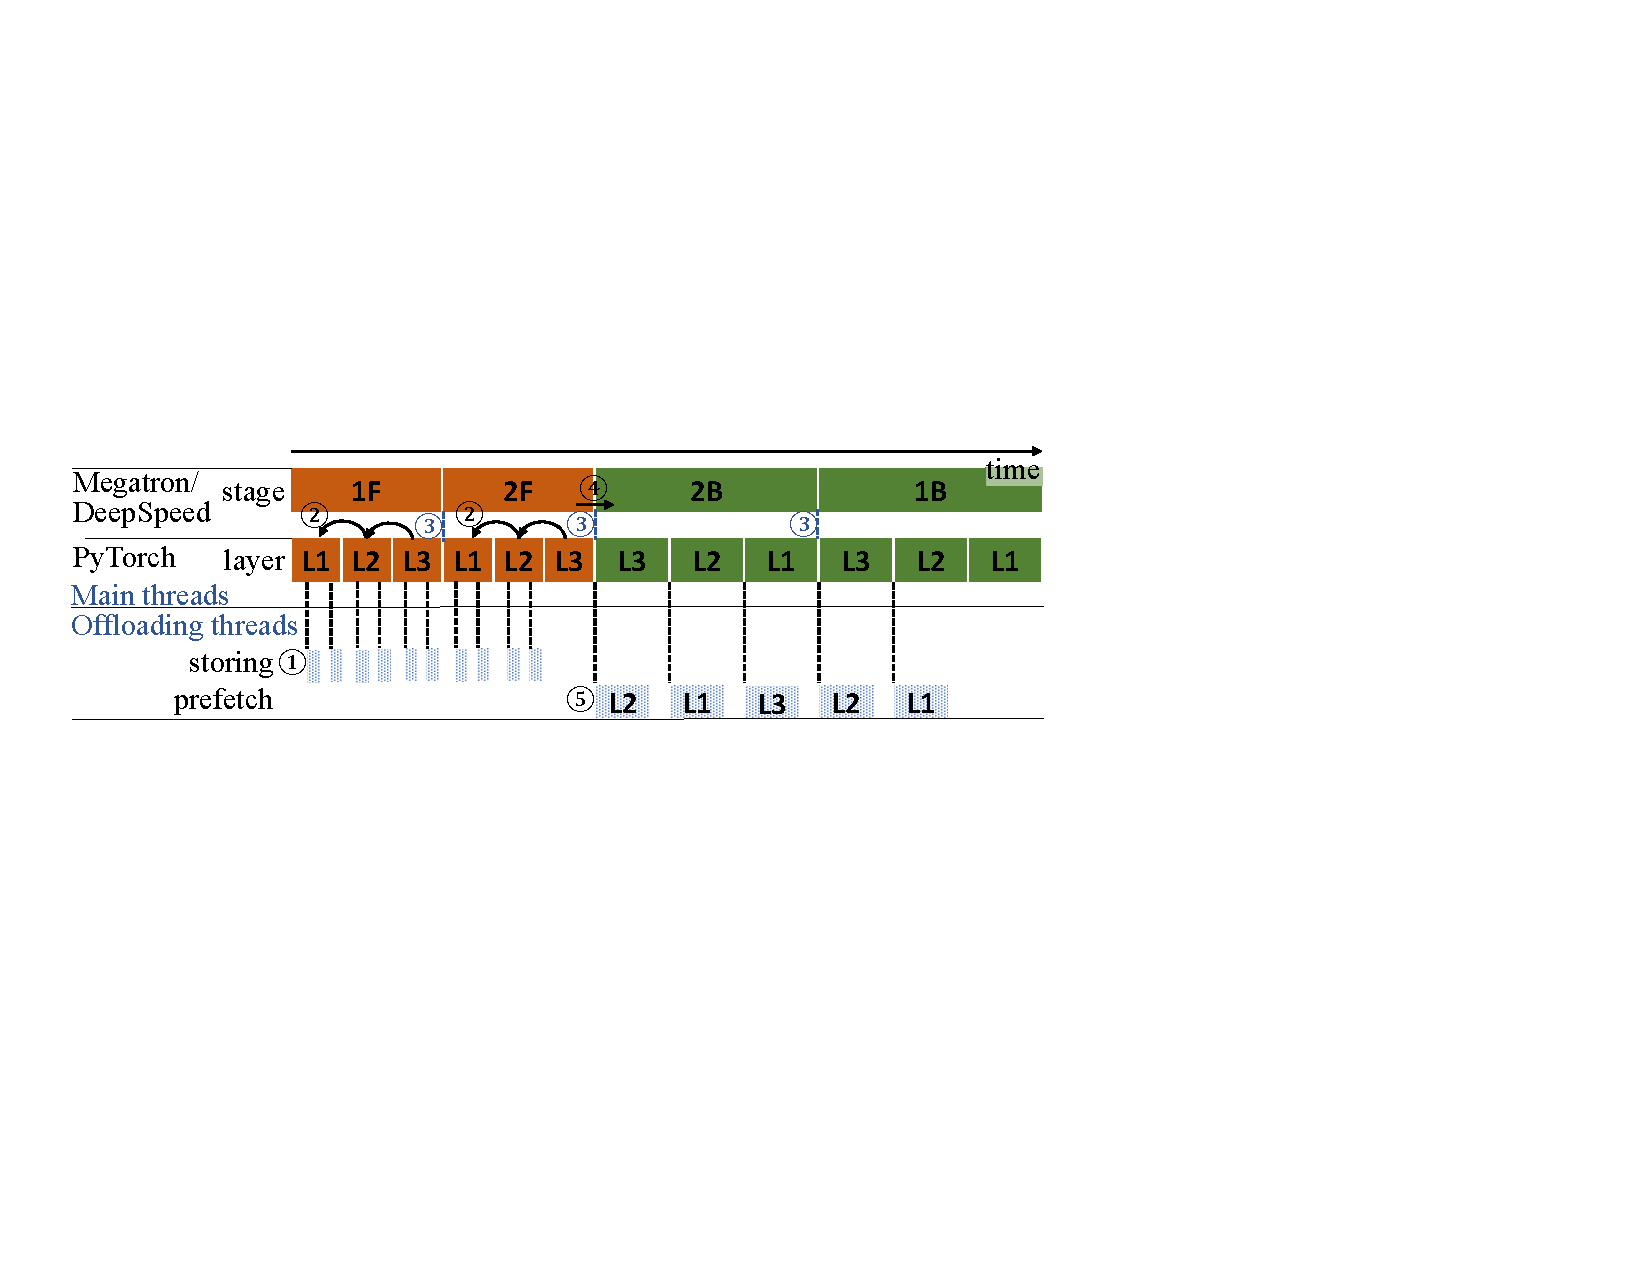
\includegraphics[width=\linewidth]{figures/SSDTrain/Pipe.pdf}
\caption{\label{fig:pipe}SSDTrain timeline of a step of a two-micro-batch three-layer (L) model. PyTorch hooks are used to trigger tensor cache bookkeeping, tensor offloading (\textcircled{1}), and tensor loading (\textcircled{5}). In the forward (F) propagation, SSDTrain records the order of scopes (\textcircled{2}) and switches between micro-batches at the end of the stages (\textcircled{3}). SSDTrain starts loading when it is switched to the backward (B) propagation (\textcircled{4}). }
\end{figure}

Figure~\ref{fig:software_arch} shows the SSDTrain software components. 
The tensor cache manages the activations and performs tensor offloading and loading. To achieve this, PyTorch hooks are used to alter PyTorch execution. Section~\ref{sec:tensor_cache} details the design and implementation of the tensor cache. SSDTrain has the SSD offloader that targets NVMe SSDs within the same node and the CPU offloader that targets host memory. Each offloader encapsulates the logic to transfer CUDA tensors to and from an offloading target. The SSD offloader leverages the GDS python binding, kvikio~\cite{nvidiaRapidsaiKvikioKvikIO2022}. Using the \texttt{LD\_PRELOAD} library interposition mechanism, CUDA malloc hook is a shared library that alters CUDA memory allocation and free API calls so that the memory is properly registered and deregistered for best GDS performance. This allows us to keep the PyTorch CUDA cached memory allocator for easy comparison with the baseline, without replicating its implementation in a PyTorch pluggable memory allocator or modifying the PyTorch runtime C++ code. The CPU offloader is for future work on clusters with massive remote SSD storage. It is backed by an allocator with pre-allocated host-pinned memory. The pool size is determined by profiling the first training step. New API calls are added to Megatron's and DeepSpeed's schedulers so that the tensor cache could get hints about stage changes and micro-batch changes, e.g., \textcircled{3} and \textcircled{4} in Figure~\ref{fig:pipe}. The following paragraph details hinted DeepSpeed's scheduler as an example.

To use SSDTrain, moderate code additions are needed in the existing script: \texttt{configure\_tensor\_cache()} in Algorithm~\ref{algo:tensor_cache_configure} shows the logic to configure tensor cache before training. The logic registers the PyTorch hooks, bookkeeps the parameters to not offload them when they are registered onto the computational graph, and monkey-patches~\cite{wikipediaMonkeyPatch2024} the schedulers. 
With the dynamicity of PyTorch, monkey-patch overrides a defined function by assigning the custom implementation to the defined \kwc{function} in a package. \texttt{deepspeed\_exec\_schedule()} shows the hints added to DeepSpeed's pipeline scheduler. Before and after the execution of each command, APIs are called to notify the tensor cache about the upcoming stage~(line 13) and the completion of an action~(line 15). Accordingly, the tensor cache can prefetch data or wait for I/O to complete. Megatron's scheduler is patched similarly.
 
SSDTrain extends naturally to distributed settings such as use with ZeRO, because frameworks like DeepSpeed and Megatron divide the workload into processes built on top of PyTorch's built-in tensor functionality.
By working below PyTorch and keeping each process' activities local, SSDTrain applies directly to distributed launches.





\subsection{Hook-Based Implementation of Tensor Cache}
\label{sec:tensor_cache}

To benefit from tensor offloading, the GPU memory that the offloaded tensors own must be released when the tensors are not in use. However, by default, PyTorch stores a reference to all the activations on the computational graph, disallowing the GPU memory to be reclaimed. The tensor cache alters the PyTorch execution so that the identifiers, not the references, of the activations are registered on the computational graph; upon PyTorch's reusing the activation tensor, the tensor cache uses the identifier from the computational graph as the key to return the requested tensor. In forward propagation, when the tensor finishes offloading, the tensor cache no longer holds a reference to it, allowing its memory to be reclaimed by Python garbage collection once the Python control flow gets out of the function scope where the tensor object is used. In the backward propagation, the tensor cache holds a reference to the tensor by loading it from the SSD before its use; when all the module scopes the tensor is referred to have been finished, the reference is no longer held, allowing its memory to be reclaimed.


In short, the tensor cache is the in-memory structure that manages the references to all activations and keeps track of activations' states, including whether they are being offloaded, the path in the file system, etc. 


As Algorithm~\ref{algo:tensor_cache_hooks} shows, the tensor cache relies on the three PyTorch hook pairs to alter its execution behavior.


The forward hook pair works in the forward propagation: The start of a module triggers the forward pre-hook, and the finish of a module triggers the forward hook. 
The tensor cache maintains the current scope stack using the forward hook pair: Upon entrance to a module, the module is pushed to the stack;
when the module exits, it is popped out.

The backward hook pair is similar. 
When entering a module, the tensor cache prefetches activations in upcoming modules. Section~\ref{sec:prefetch} details prefetching.
When exiting a module, the tensor cache removes it from the scope lists of all activations. Activations no longer in use are removed, whose memory will be released by garbage collection.


\begin{figure}[!t]
\centering
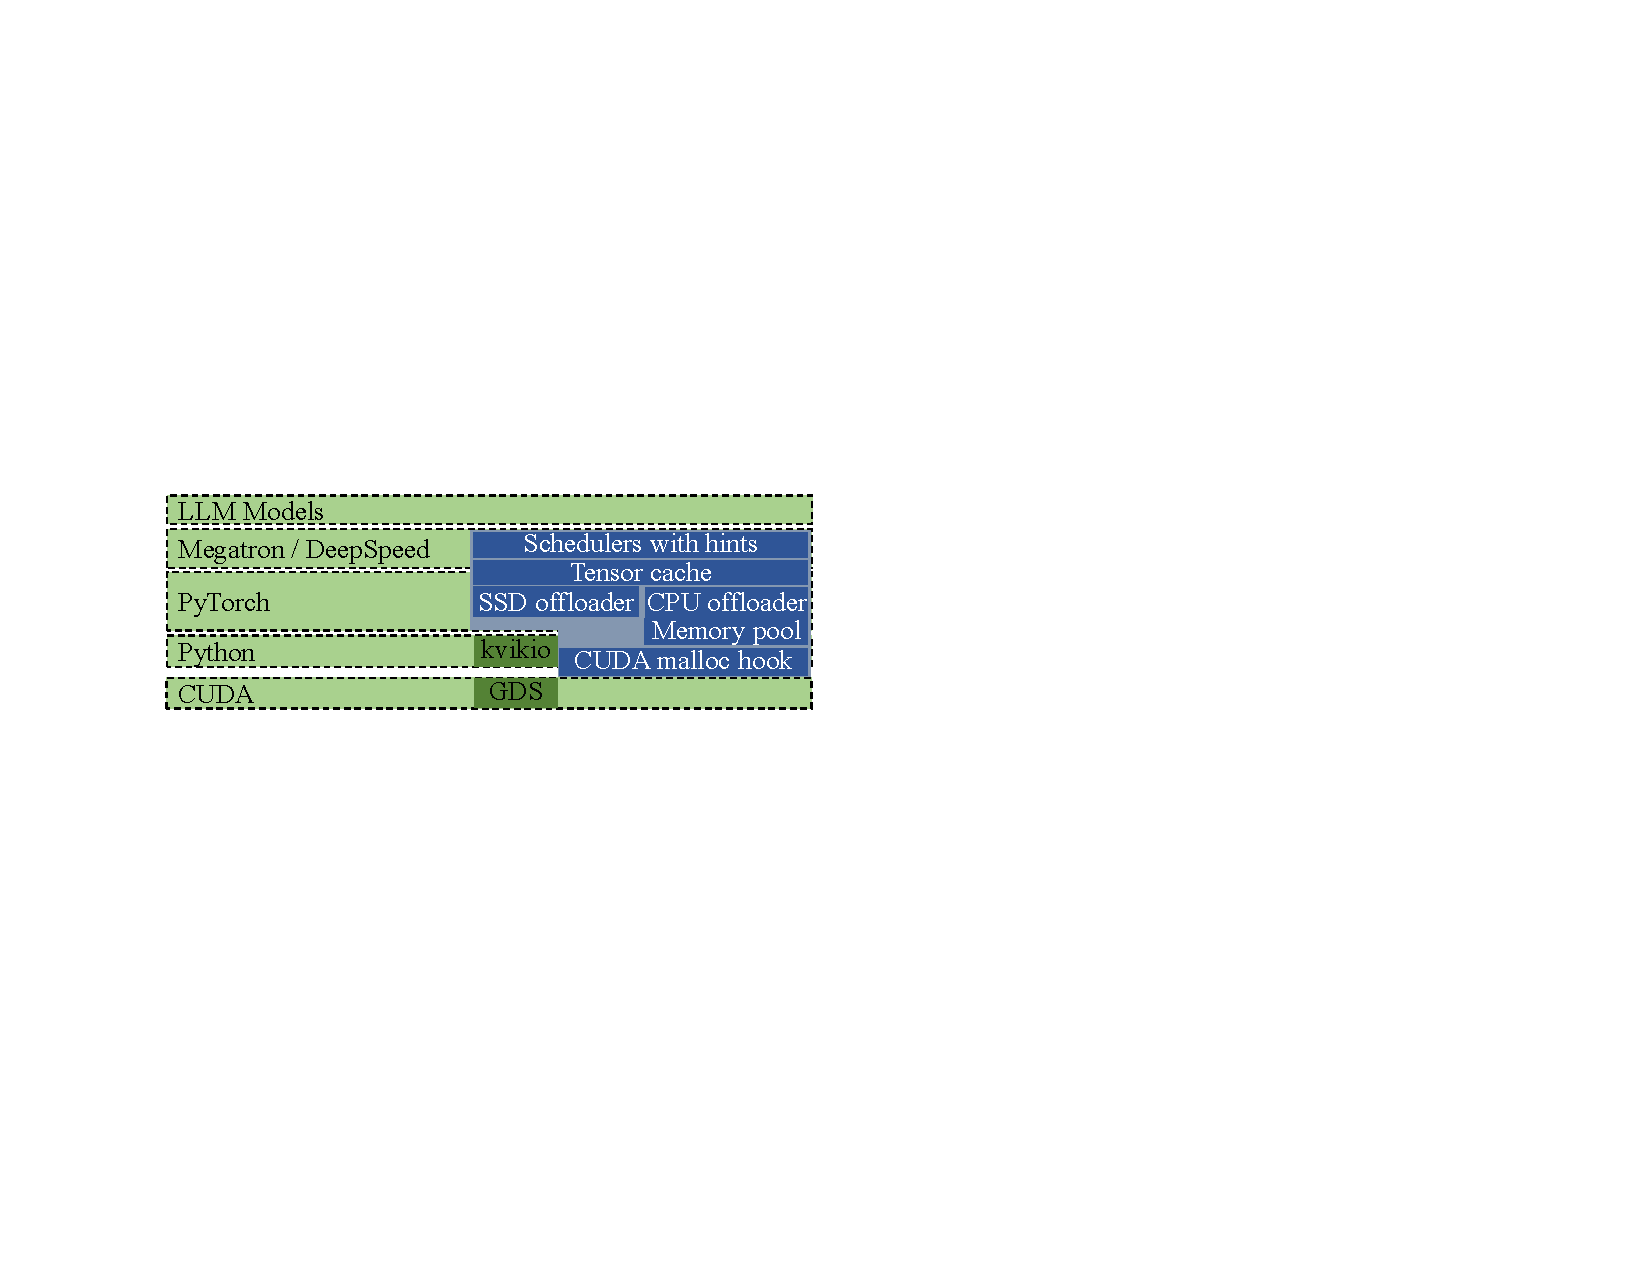
\includegraphics[width=0.85\linewidth]{figures/SSDTrain/software_arch_v2.pdf}
\caption{\label{fig:software_arch} SSDTrain software architecture. The components of SSDTrain are shown as blue blocks with white text. The CUDA malloc hook is a C++ library, while others are Python code.}
\end{figure}




\begin{algorithm}[!t]
{
\DontPrintSemicolon
    \KwIn{The tensor cache \texttt{tcache} and the LLM model \texttt{model}.}
    \SetKwFunction{FConf}{\texttt{configure\_tensor\_cache}}
    \SetKwProg{Fn}{Function}{:}{}
    \Fn{\FConf{\texttt{tcache}, \texttt{model}}}{
        \texttt{tcache.register\_hooks()}
        
        \For{\texttt{param in model.parameters()}}{
            \texttt{tcache.register\_parameters(param)}
        }

        Monkey-patch DeepSpeed's and Megatron's schedulers. 
    }

    \SetKwFor{For}{{\color{blue}for}}{{\color{blue}:}}{}
    \SetKwFunction{FSched}{\texttt{deepspeed\_exec\_schedule}}
    \Fn{\FSched{\texttt{self}, \texttt{schedule}}}{
        \For{{\color{blue}\texttt{step\_cmds in schedule}}}{
            \For{{\color{blue}\texttt{idx\_cmd, cmd in enumerate(step\_cmds)}}}{                
                \texttt{tcache.set\_stage(cmd)}

                \texttt{nxcmd = get\_next(idx\_cmd, step\_cmds)}
                
                \texttt{tcache.set\_next\_stage(nxcmd)}

                \If{\texttt{cmd} is communication and \texttt{nxcmd} is backward pass}{
                    \texttt{tcache.prefetch\_last\_module()} 
                }

                {\color{blue}\texttt{self.execute(cmd)}}

                \lIf{\texttt{cmd} is a backward pass}{
                \texttt{tcache.wait\_IO()}
                }
            }
        }
    }
}
\caption{Logic to configure tensor cache before training and DeepSpeed scheduler logic with tensor cache hints. The original code before adding hints is blue. As shown, changes to adopt tensor cache are moderate.}
\label{algo:tensor_cache_configure}
\end{algorithm}

When a tensor is to be registered onto the computational graph, the pack hook is called to produce a value to be registered instead.
When the tensor is reused, the unpack hooks are called to take in the object on the computational graph and return the original tensor.
Figure~\ref{fig:hooks} illustrates the tensor cache's activity when triggering the pack or unpack hook.
When the multiply operator $\texttt{x}\cdot\texttt{w}$ finishes (\textcircled{1}), the pack hook is called~(\textcircled{2}) on the input \texttt{x} and parameters \texttt{w}.
Tensor cache has a record of parameters and accordingly returns \texttt{w} to let it be registered on the graph as is.
The tensor will also be returned as is if the tensor is on CPU or it is too small~(line 12 in Algorithm~\ref{algo:tensor_cache_hooks}).
As line 16 in Algorithm~\ref{algo:tensor_cache_hooks} shows, the tensor cache does not offload tensors but only keeps a record when the module is to be kept in the memory or in backward propagation.
The first condition holds true when the adaptive offloading algorithm determines to keep the last few modules in GPU memory~(Section~\ref{sec:adaptive}).
The second condition is true when an activation-checkpointing-enabled function does recomputation in the backward propagation to reproduce the activations.
For tensor \texttt{x} in Figure~\ref{fig:hooks}, the tensor cache stores it to the SSDs~(\textcircled{3}) and returns a tensor identifier.
When the unpack hook is triggered~(\textcircled{B}), in the backward propagation~(\textcircled{A}), the tensor cache either waits until the prefetch finishes(\textcircled{C}), and eventually returns the tensor. 

\subsection{Deduplicating Tensors and Excluding Parameters}

Tensor cache has a \texttt{get\_id()} \kwc{method} to assign a unique identifier to each tensor.
The shortcoming of PyTorch native \texttt{id()} is that its returned value is related to the GPU memory address. As SSDTrain offloads activations, the latter will be cleared by garbage collection once the control flow goes out of its use scope.
The GPU memory address may be reused, causing identifier collision. 
To solve this, \texttt{get\_id()} combines the timestamp when it first processes the tensor with the tensor shape as the unique identifier. When \texttt{get\_id()} processes a tensor \texttt{t} for the first time, \texttt{get\_id()} adds the current timestamp as an additional attribute to the tensor's underlying storage \texttt{t.untyped\_storage()} instead of \texttt{t}.
This is because sometimes PyTorch creates new \texttt{torch.Tensor} objects representing the identical tensor.
All future \texttt{get\_id()} calls get the attribute value.
This deduplicating scheme helps prevent redundant I/Os.

PyTorch registers all needed tensors in backward propagation into the computational graph, including activations and parameters. As SSDTrain focuses on offloading activations, the tensor cache excludes the model parameters. To achieve this, before training, the tensor cache records the identifiers of all model parameters~(line 4 in Algorithm~\ref{algo:tensor_cache_configure}). As linear layers store the transpose of the parameter tensors for backward propagation, the unique identifiers of the transpose are recorded. One benefit of our \texttt{get\_id()} scheme is that the identifier for the transpose of the same parameter tensor remains consistent across steps. This is because the transpose uses the original tensor's underlying storage, to which we already assigned a timestamp before training.


\subsection{Offloading and Forwarding Tensors}
\label{sec:prefetch}

The tensor cache has two thread pools---one for storing tensors and the other for loading tensors. The jobs submitted to each thread pool are executed in first-in-first-out~(FIFO) order.

To hide the I/O latency, the tensor cache starts prefetching each activation before the corresponding module's backward propagation. 
The activations in the last module are kept in GPU memory, so they need not be prefetched.
This simple scheme suffices because, in PyTorch, the CPU submits GPU kernel launches and memory operations ahead of GPU execution. Prefetching schemes are equivalent as long as there are always I/O tasks in the GPU job queue to keep PCIe busy.



Upon loading a tensor, if it is still being stored, the tensor cache will return its original in-memory reference to skip loading from SSD. We call this data forwarding. For example, in Figure~\ref{fig:hooks}, when the PyTorch engine retrieves tensor \texttt{x} from the \texttt{MulBWD} node, if it is still being stored to the SSDs, it is in memory. Instead of loading the tensor, the tensor cache returns its in-memory reference by converting the weak reference to a reference and storing the obtained reference in the tensor cache for the future if it is used in other scopes.



\begin{figure}[!t]
\centering
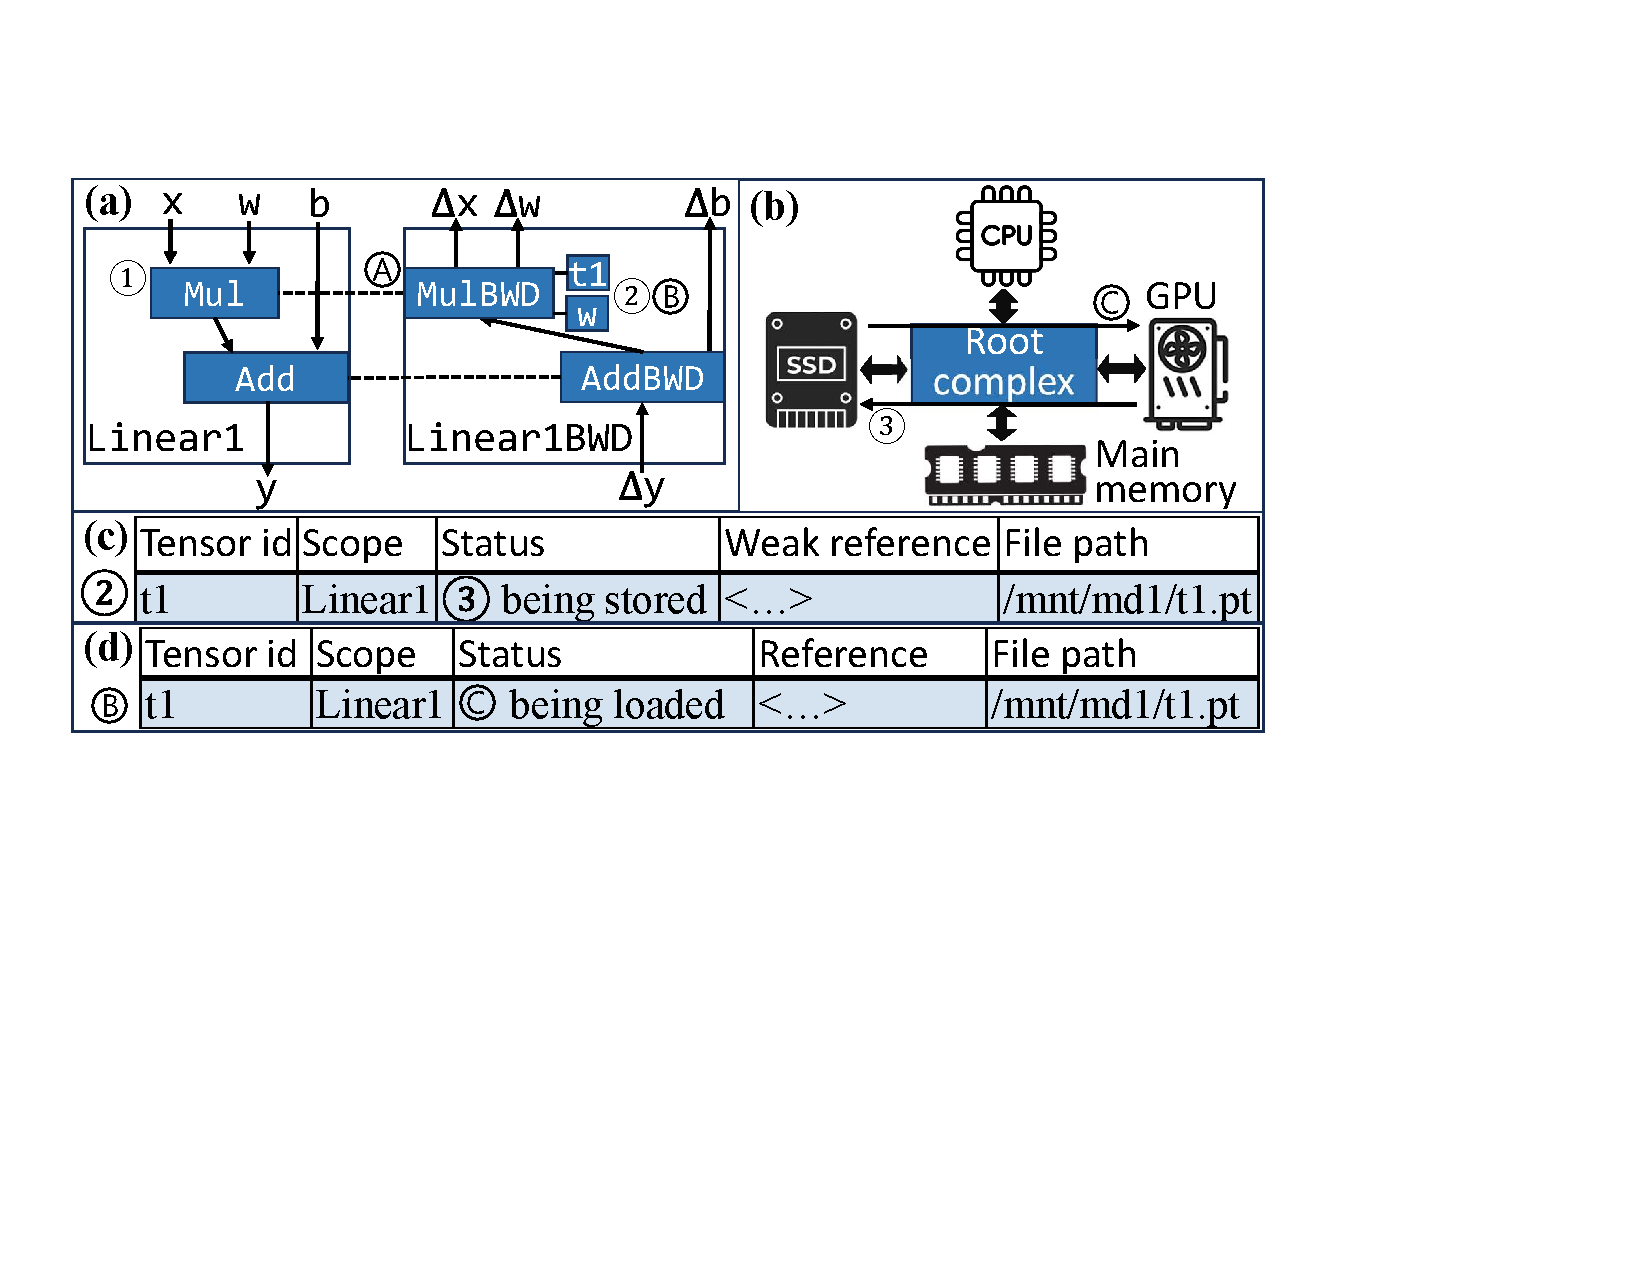
\includegraphics[width=0.91\linewidth]{figures/SSDTrain/hooks.pdf}
\caption{\label{fig:hooks} Tensor cache registers pack--unpack hook pair to offload tensors and reload tensors. \textbf{(a)} shows the PyTorch computational graph. \textbf{(b)} shows the hardware data path. \textbf{(c)} and \textbf{(d)} show the tensor cache state when the pack or unpack hook is triggered. During an operator~(\textcircled{1}), PyTorch calls the pack hook with tensors to be saved for backward propagation and registers the return values on the computational graph~(\textcircled{2}). Tensor cache tracks the tensors, offloads them~(\textcircled{3}), and returns identifiers for the tensors. In an operator~(\textcircled{A}) in the backward propagation, PyTorch calls the unpack hook with the identifiers to get tensors~(\textcircled{B}). The tensor cache blocks until the requested tensors are loaded in GPU memory~(\textcircled{C}). }
\end{figure}


\begin{algorithm}[!t]
{
\DontPrintSemicolon
    \KwIn{The tensor cache \texttt{tcache}, current scope \texttt{module}, tensor to pack \texttt{tensor}, and/or object to unpack \texttt{obj}.}
    \SetKwProg{Fn}{Function}{:}{}
    \SetKwFunction{FFPH}{\texttt{forward\_pre\_hook}}
    \Fn{\FFPH{\texttt{module}}}{ 
    Add \texttt{module} to \texttt{tcache}'s current scope stack.
    
    
    }
    \SetKwFunction{FFH}{\texttt{forward\_hook}}
    \Fn{\FFH{\texttt{module}}}{ 
    Pop \texttt{tcache}'s innermost scope from the current scope stack.

    
    }
    \SetKwProg{Fn}{Function}{:}{}
    \SetKwFunction{FBPH}{\texttt{full\_backward\_pre\_hook}\textsuperscript{*}}
    \Fn{\FBPH{\texttt{module}}}{ 
    Prefetch the tensors in the next module.
    
    }
    \SetKwFunction{FBH}{\texttt{full\_backward\_hook}\textsuperscript{*}}
    \Fn{\FBH{\texttt{module}}}{ 
    \For{each tensor \texttt{t} in \texttt{module} tracked by \texttt{tcache}}{
            Remove \texttt{module} from \texttt{t}'s record.

            Release and stop tracking \texttt{t} if no scope is using \texttt{t}.
        }
    }
    \SetKwFunction{FPCKH}{\texttt{pack\_hook}}
    \Fn{\FPCKH{\texttt{tensor}}}{
     \lIf{\texttt{tcache.is\_parameter(tensor) or tensor.is\_cpu or math.prod(tensor.size())<2**20}}{
     \Return{\texttt{tensor}}
     }
     
    
    \texttt{tid = get\_id(tensor)}

    \texttt{tcache.add\_to\_current\_scope(tid)}

    \If{\texttt{tcache.is\_current\_scope\_kept\_in\_memory() or tcache.is\_current\_in\_backward()}}{
     \texttt{tcache.keep\_in\_gpu\_memory(tid,tensor)}
     }\lElse{
     \texttt{tcache.offload(tid,tensor)}
     }
    
    
    \Return{\texttt{tid}}
    }

    \SetKwFunction{FUPCKH}{\texttt{unpack\_hook}}
    \Fn{\FUPCKH{\texttt{obj}}}{
        \lIf{\texttt{isinstance(obj,torch.Tensor)}}{
            \Return{\texttt{obj}}
        }
        \lIf{\texttt{not tcache.is\_loaded(obj)}}{
        \texttt{tcache.load\_or\_wait\_load(obj)}
        }
        \Return{\texttt{tcache.get\_loaded\_tensor(obj)}}
    }
}
\caption{Tensor cache registers PyTorch hooks to trigger actions during training.}
\label{algo:tensor_cache_hooks}
\begin{flushleft} \footnotesize * PyTorch added \texttt{full\_} prefix to the backward hook pair APIs to distinguish the current reworked design from the superseded one.
\end{flushleft}
\end{algorithm}


\begin{figure}[!t]
\centering
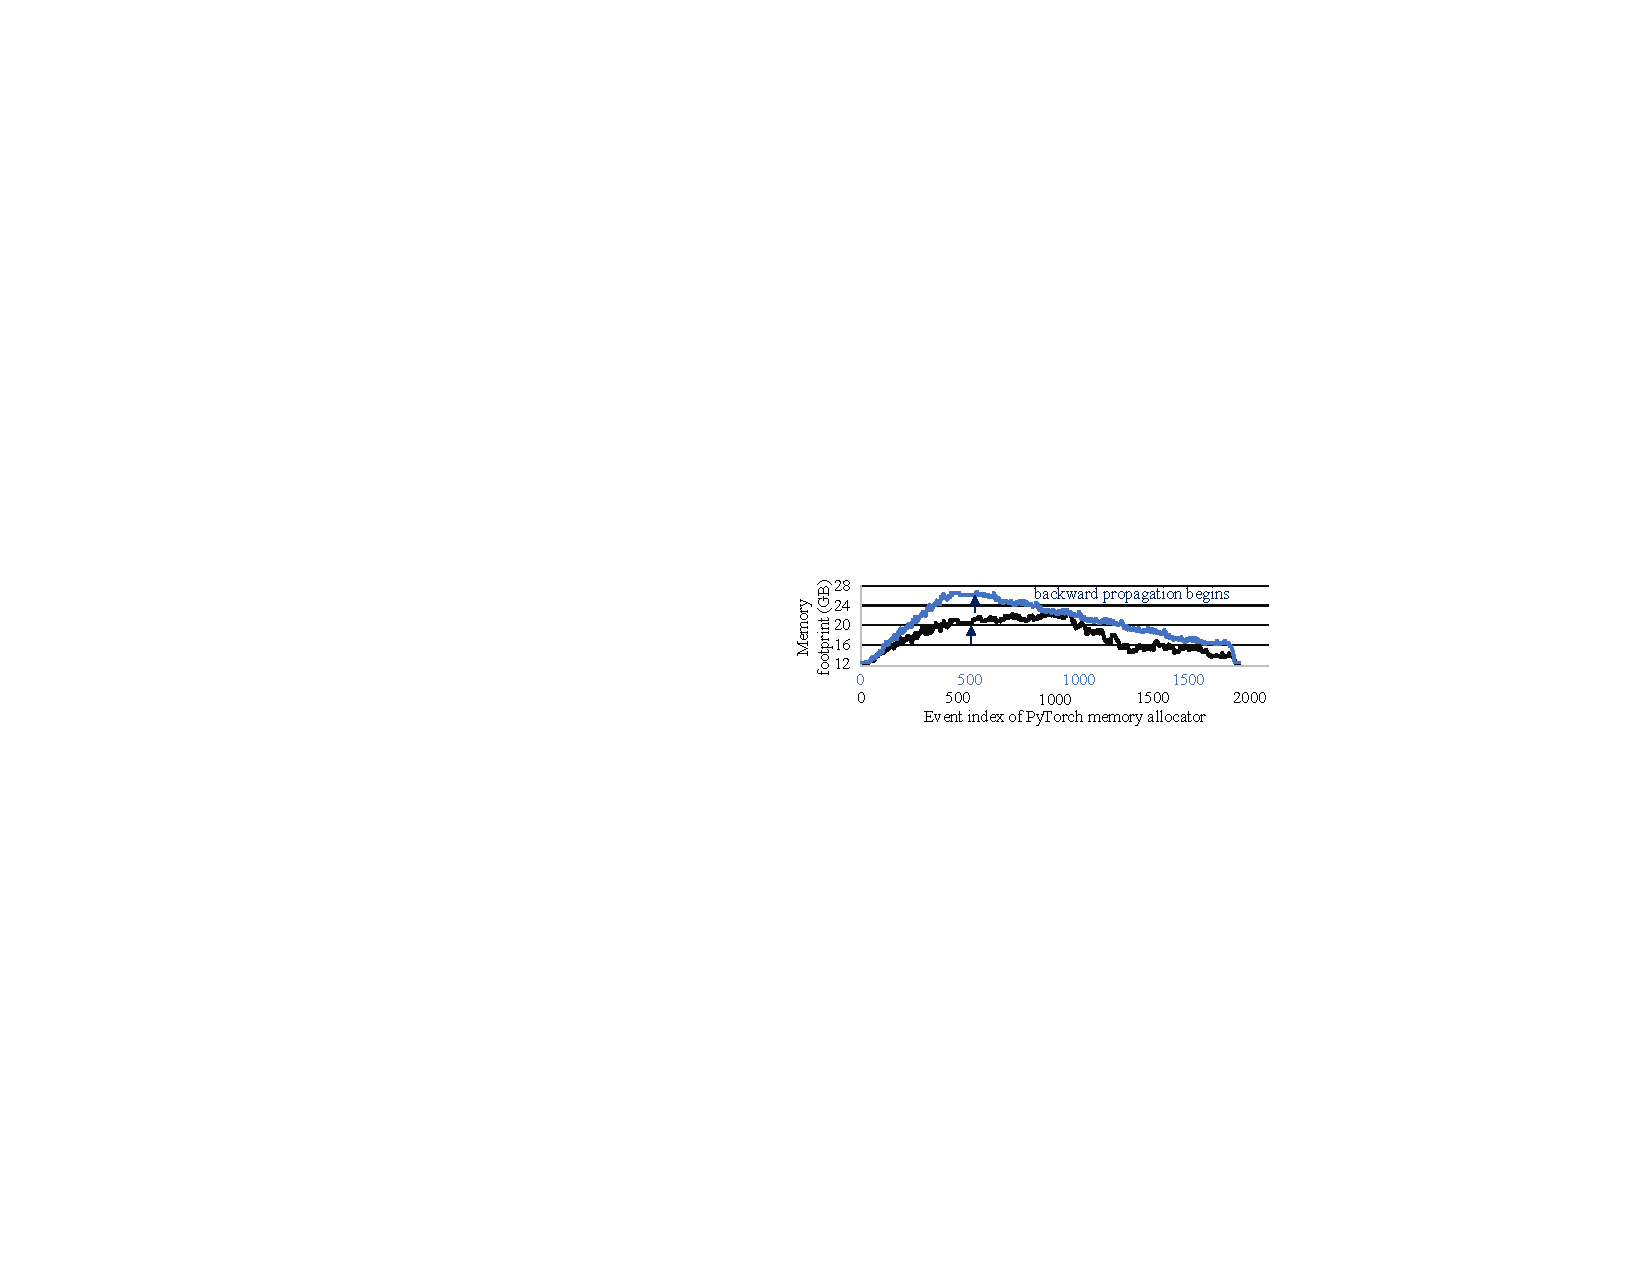
\includegraphics[width=0.9\linewidth]{figures/SSDTrain/snapshot_aligned_2.pdf}
\caption{\label{fig:snapshot} Memory footprint of one A100 in a BERT training step with offloading~(black) and without~(blue) on Table~\ref{tab:configurations}'s system. Run with offloading incurs more allocator events because of memory release and allocation caused by tensor offloading and reloading. SSDTrain reduces memory footprint at the beginning of backward propagation by 45\% and end-to-end peak memory footprint by 25\%.}
\end{figure}


\begin{figure}[!t]
\centering
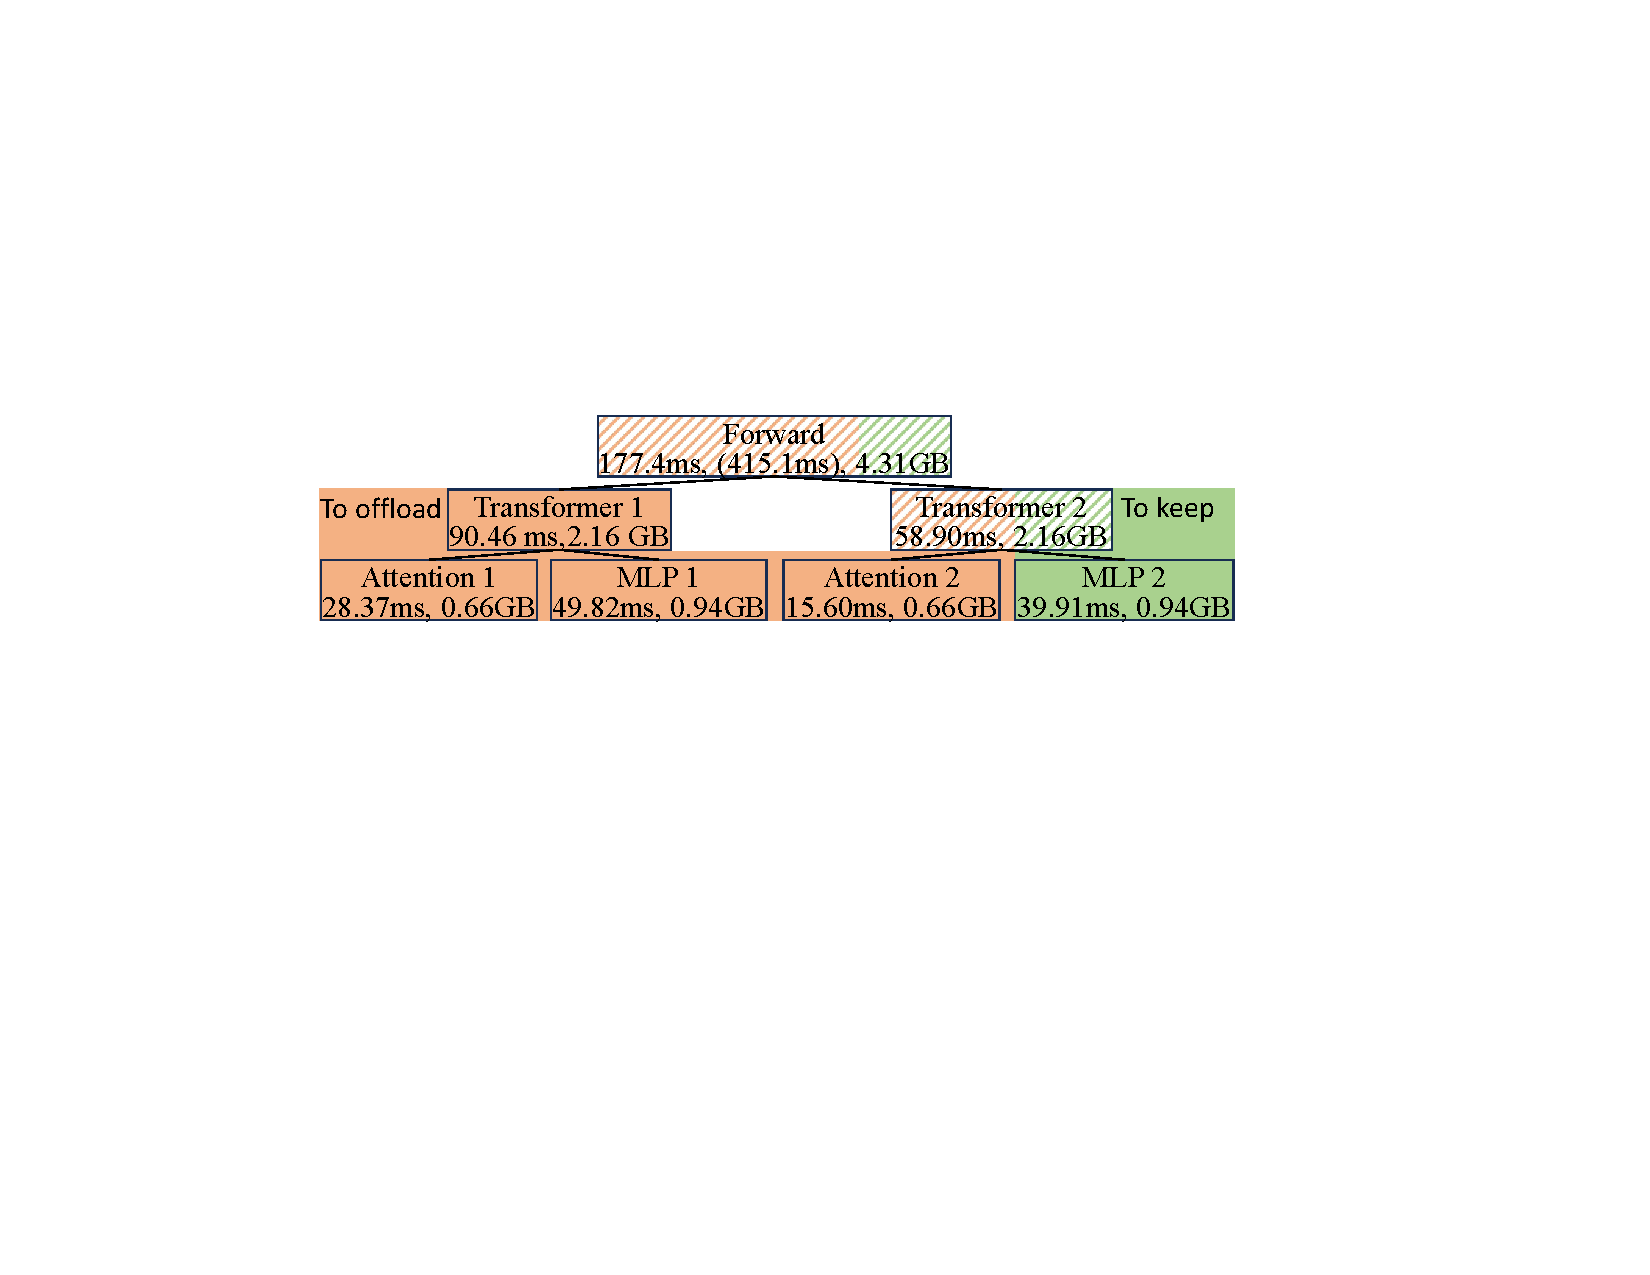
\includegraphics[width=0.95\linewidth]{figures/SSDTrain/adaptive.pdf}
\caption{\label{fig:adaptive} The adaptive offloading algorithm uses profiling to decide modules in which the activations are to be kept in GPU memory. The model is represented as a tree where each scope is a node. On each node, the forward computation time and data transfer size are recorded during profiling. The I/O time in the forward propagation is also recorded and shown in parenthesis in the root node.}
\end{figure}


\begin{figure}[!t]
\centering
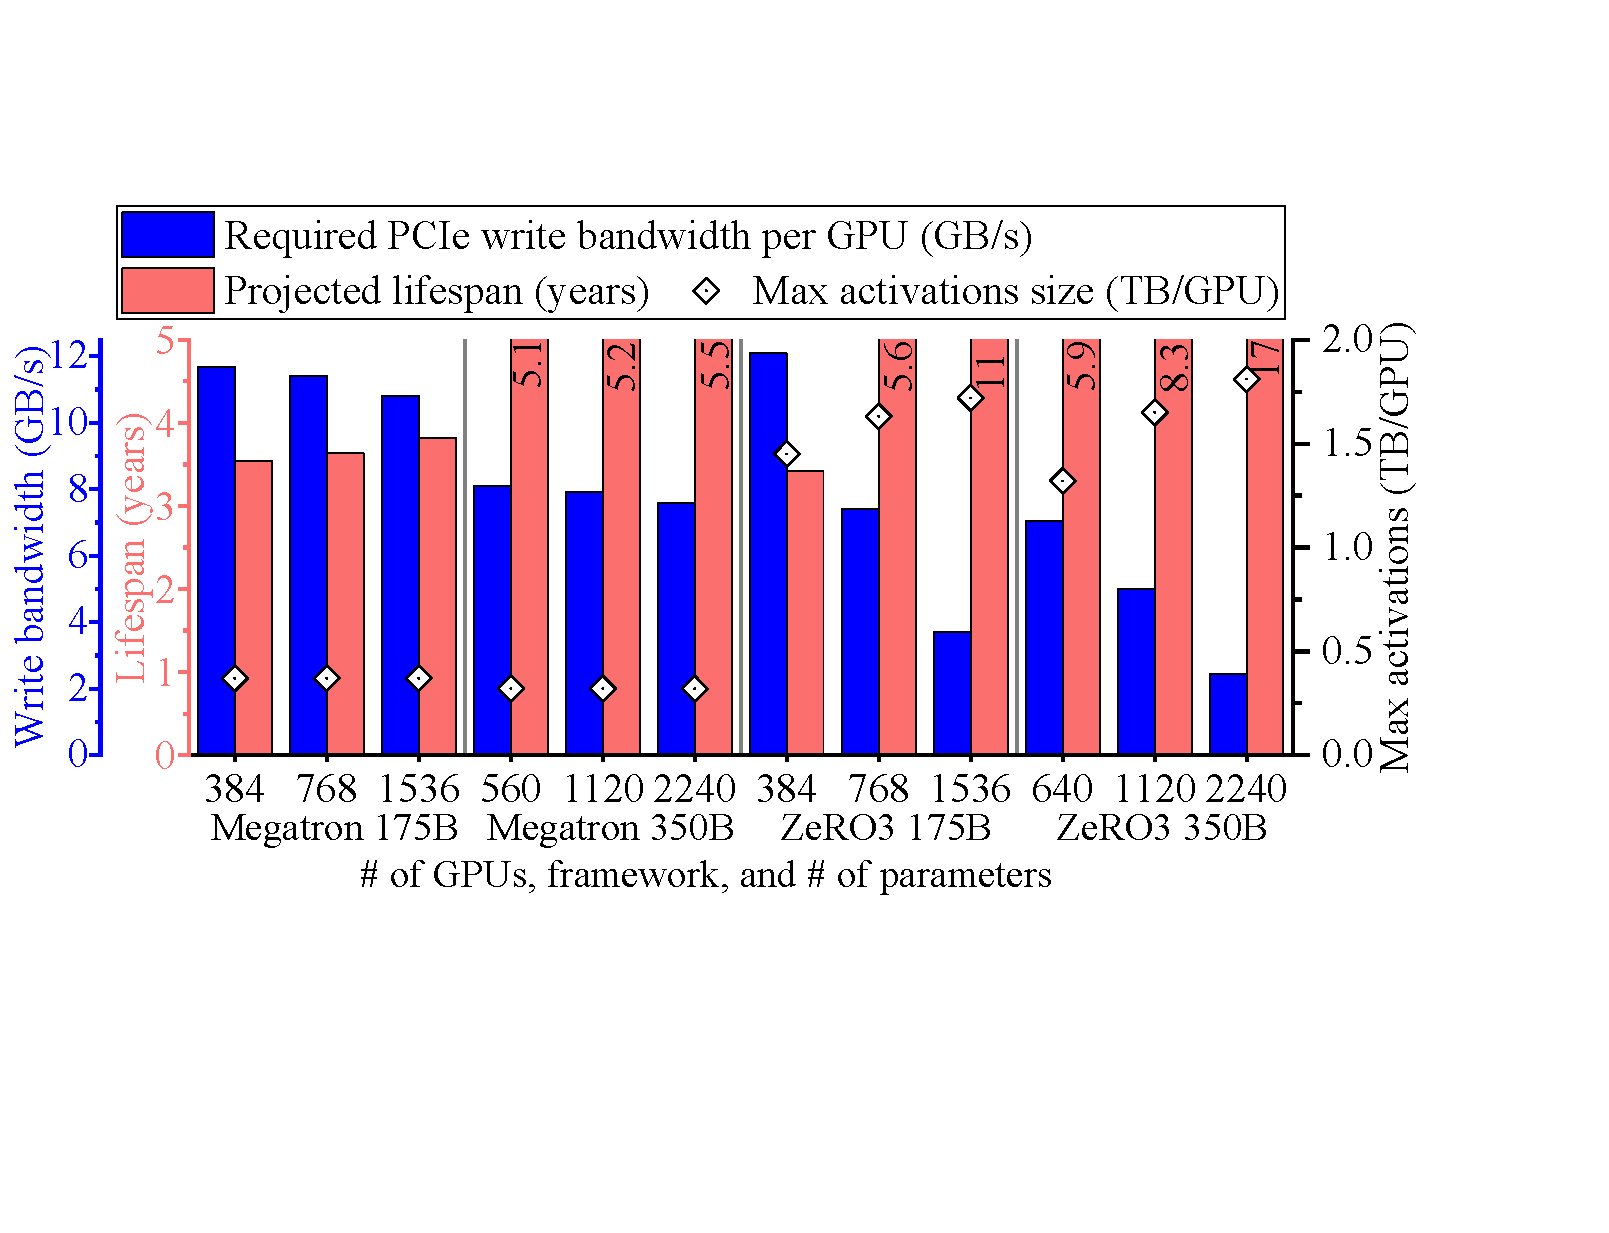
\includegraphics[width=0.95\linewidth]{figures/SSDTrain/ProjectedPerfModel3.pdf.pdf}
\caption{\label{fig:projected_perf_model} Estimate of SSD lifespan~(left pink vertical axis), PCIe write bandwidth~(left blue vertical axis) and maximal activations size per GPU~(right vertical axis). Lifespans longer than 5 years are shown on top of the pink bars. The horizontal axis shows the number of GPUs, the framework, and the model size~\cite{shoeybiMegatronLMTrainingMultiBillion2020a}. ZeRO3 stands for DeepSpeed with stage-3 ZeRO, i.e., all optimizer states, gradients, and parameters are sharded \kwc{across data parallel ranks}.}
\end{figure}



\subsection{Adaptive Offloading}
\label{sec:adaptive}

One insight we got during SSDTrain is that the activation offloading should target minimizing the peak memory usage so that the same system could accommodate a configuration with larger activations without triggering out-of-memory~(OOM) errors. Offloading tensors after the peak is not helpful. In Figure~\ref{fig:snapshot}, the \kwc{blue} curve is the memory footprint without offloading; it illustrates that GPU memory usage peaks at the beginning of the backward propagation. The \kwc{black} curve shows the memory footprint with offloading, where the peak is delayed by the in-progress offloading jobs and new intermediate tensors created in backward propagation. Excessive tensor offloading may keep the tensor reference even after its last use in backward propagation, delaying the reclamation of its memory. To reduce unnecessary offloading after the peak, we devised adaptive offloading with two features.

First, when a thread is assigned a storing job, the thread will check if the tensor was forwarded. If so, the job will be canceled. Second, as illustrated in Figure~\ref{fig:adaptive}, we devise an algorithm to choose a module from which the offloading is paused. We profile a step to collect: (1) the data transfer size and computation time of each MLP block and attention block, and (2) the forward propagation's computation time, data transfer time, and total data transfer amount. Suppose module $m$ is the last module to offload in a step. The required data transfer bandwidth is to finish offloading for all the modules before $m$ and both offloading and reloading for module $m$ by the time the backward propagation of module $m$ begins. With the estimate that the backward propagation time is twice the forward propagation time, the required data transfer bandwidth can be calculated by the collected numbers. It should be no larger than the write bandwidth in the measured forward propagation.






\subsection{SSD Write Amount, Bandwidth, and Lifespan}
\label{sec:projected_life}
To confirm whether our design is viable in large-scale training systems, particularly regarding SSD endurance and required bandwidth, we conduct performance modeling to obtain the forward propagation time per training step and the size of activations produced in the process. 

We extend the performance model package \texttt{llm-analysis}~\cite{liLLMAnalysisLatencyMemory2023}.
To estimate the forward propagation time, \texttt{llm-analysis} models each transformer layer as a simple pipeline, 
$t= \max\left(\sum_{l}\max\left(t_{l,compute}, t_{l,memory}\right), t_{ZeRO,communicate}\right)$,
where $l$ denotes any layers inside a transformer layer. When ZeRO is enabled, the ZeRO communication time is assumed to be perfectly pipelined with the non-ZeRO computation and memory operations at the level of the transformer layer. 

 We model the required PCIe write bandwidth per GPU as the total amount of activations divided by half the training time. As Section~\ref{sec:adaptive} explains, some activations may be written at the early stages of the backward propagation to reduce the needed PCIe bandwidth. We also assume that the training step time $t_{step}$ is three times the forward propagation time. The lifespan is then projected as $t_{life} = S_{endurance}\cdot t_{step}/S_{activations}$ where $S_{endurance}$ is the lifetime writes allowed by the SSD endurance rating, and $S_{activations}$ is the size of activations per training step. We validated the $S_{activations}$ formula with profiled activations size in experiments in Section~\ref{sec:evaluation}. We assume four Solidigm D7-P5\kwc{620} 12.8TB~(Table~\ref{tab:ssd}) for each GPU and assume the WAF is 2.5 in JESD rating and 1 in our scenario.

With these, we obtain Figure~\ref{fig:projected_perf_model}. We use the system configurations and measured floating point throughput from Megatron-LM~\cite{shoeybiMegatronLMTrainingMultiBillion2020a}. The GPUs are A100 PCIe. Among all cases, the projected lifespan is over three years, and the PCIe write bandwidth per GPU is no greater than 12.1 GB/s.
Moreover, when the system size scales up, the required PCIe write bandwidth reduces, and the projected lifespan increases. This occurs because larger systems imply increased communication overhead and reduced computation efficiency, thus slowing down training iterations on each GPU. \kwc{Similar effects are observed when the model size scales up because larger model size leads to longer compute latency with increased 
data reuse and therefore less bandwidth requirement. Section~\ref{sec:discussion} discusses the effect of scaling up in detail. }

We also estimate the maximal size of activations each GPU produces in one step: We compute the maximal micro-batch size by assuming only two layers in a row are in GPU memory at the same time while all other activations are offloaded. Then, the activation maximal micro-batches produce in a step are the largest activations offloading could open up, which are shown as diamond marks in Figure~\ref{fig:projected_perf_model}. The maximal activations size per GPU ranges from 0.4 TB to 1.8 TB, while the micro-batch size ranges from eight to 32. Activations so large can no longer be held by the main memory~(Figure~\ref{fig:current_sys}), and therefore, SSD is the only choice as an offloading target.



To further increase SSD endurance, the data retention period can be relaxed: NAND flash gets \kwc{86}$\times$ P/E cycles when the data retention period is relaxed from three years to \kwc{one} day~\cite{caiFlashCorrectandrefreshRetentionaware2012,yucaiErrorPatternsMLC2012,liuOptimizingNANDFlashBased2012,kimBehemothFlashcentricTraining2021}. This technique was not leveraged in the reasoning of this subsection, but we discuss its impact on cost in Section~\ref{sec:discussion}.

